\documentclass{article}
\usepackage{cmap}
\usepackage[utf8]{inputenc}
\usepackage[english,ukrainian]{babel}
\usepackage{graphicx}
\usepackage{geometry}
\usepackage{listings}
\usepackage{float}
\usepackage{amsmath}
\geometry{
	a4paper,
	left=20mm,
	right=20mm,
	top=15mm,
	bottom=15mm,
}
\lstset{
	language=c,
	tabsize=4,
	keepspaces,
	showstringspaces=false,
}
\graphicspath{ {./pictures} }
\setlength{\parindent}{4em}

\newcommand\subject{Основи електроніки}
\newcommand\lecturer{професор кафедри ПЗ \\ Фечан А.В.}
\newcommand\teacher{доцент кафедри ПЗ \\ Коцун В.І.}
\newcommand\mygroup{ПЗ-22}
\newcommand\lab{1}
\newcommand\theme{Ознайомлення з програмним продуктом Multisim Live}
\newcommand\purpose{Ознайомитись з програминим продуктом Multisim Live}

\begin{document}
\begin{normalsize}
	\begin{titlepage}
		\thispagestyle{empty}
		\begin{center}
			\textbf{МІНІСТЕРСТВО ОСВІТИ І НАУКИ УКРАЇНИ\\
				НАЦІОНАЛЬНИЙ УНІВЕРСИТЕТ "ЛЬВІВСЬКА ПОЛІТЕХНІКА"}
		\end{center}
		\begin{flushright}
			\textbf{ІКНІ}\\
			Кафедра \textbf{ПЗ}
		\end{flushright}
		\vspace{200pt}
		\begin{center}
			\textbf{ЗВІТ}\\
			\vspace{10pt}
			до лабораторної роботи № \lab\\
			\textbf{на тему}: “\textit{\theme}”\\
			\textbf{з дисципліни}: “\subject”
		\end{center}
		\vspace{112pt}
		\begin{flushright}
			
			\textbf{Лектор}:\\
			\lecturer\\
			\vspace{28pt}
			\textbf{Виконав}:\\
			
			студент групи \mygroup\\
			Коваленко Д.М.\\
			\vspace{28pt}
			\textbf{Прийняв}:\\
			
			\teacher\\
			
			\vspace{28pt}
			«\rule{1cm}{0.15mm}» \rule{1.5cm}{0.15mm} 2023 р.\\
			$\sum$ = \rule{1cm}{0.15mm}……………\\
			
		\end{flushright}
		\vspace{\fill}
		\begin{center}
			\textbf{Львів — 2023}
		\end{center}
	\end{titlepage}
		
	\begin{description}
		\item[Тема.] \theme.
		\item[Мета.] \purpose.
	\end{description}

	\section*{Теоретичні відомості}
	Експериментально встановлено, що зі збільшенням електрорушійної сили
	(е. р. с.) джерела живлення при незмінному опорі в колі струм зростає
	пропорційно їй; зі збільшенням опору в колі при незмінній е. р. с. струм
	пропорційно йому зменшується, а при зменшенні опору — збільшується. Для
	всього кола ці залежності можна виразити таким рівнянням:
	
	\begin{equation}
		I = E(R+R_0)\nonumber
	\end{equation}
	\begin{flushright}
		$R$ – опір зовнішньої частини кола,\\ $R_0$ – опір внутрішньої частини кола.
	\end{flushright}

	Тобто сила струму в колі прямо пропорційна е. р. с. джерела живлення й
	обернено пропорційна сумі опорів зовнішньої та внутрішньої частин кола.
	Частина е.р.с. $Е$, що витрачається на подолання опору $R$, називається спадом
	напруги у зовнішній частині кола ($U$); друга частина цієї е.р.с., яка витрачається
	на подолання опору $R_0$, називається спадом напруг у внутрішній частині кола
	($U_0$). Таким чином
	
	\begin{equation}
		E = U + U_0 \nonumber
	\end{equation}

	Це закон Ома для всього кола. Рівняння дійсне не тільки для всього кола, а
	й для кожної його частини. Якщо розглядати лише зовнішню частину кола, то
	можна записати
	
	\begin{equation}
		I = \frac{U}{R} \nonumber
	\end{equation}

	тобто сила струму на ділянці кола прямо пропорційна спаду напруги на цій
	ділянці й обернено пропорційна її опору. Це закон Ома для ділянки кола.
	Німецький вчений Г.Р.Кірхгоф встановив закони, за допомогою яких проводять
	розрахунки струмів і напруг у розгалужених колах.
	
	\textbf{Перше правило Кірхгофа:} \textit{Алгебраїчна сума струмів, які збігаються у вузлі
	дорівнює нулю.}
	
	\begin{equation}
		\sum_{i=1}^{n}I_i=0 \equiv I_1 + I_2 + ... + I_n = I \nonumber
	\end{equation}

	\textbf{Друге правило Кірхгофа:} \textit{У будь-якому замкненому контурі розгалуженого
		кола алгебраїчна сума ЕРС дорівнює алгебраїчній сумі добутків струмів на опори
		відповідних ділянок цього контуру:}
	
	\begin{equation}
		\sum_{i=1}^{n}I_i\cdot R_i=\sum_{i}^{m}=1\nonumber
	\end{equation}
	
		\section*{Індивідуальне завдання}
	\begin{enumerate}
		\item Створити аккаунт Multisim Live.
		\item Ознайомитись з можливостями Multisim Live виконуючи кроки практичних рекомендацій.
		\item Згідно отриманого завдання провести розрахунок кола постійного струму.
		\item Згідно отриманого завдання провести розрахунок кола постійного струму.
		\item Провести перевірку попередньо розрахованих параметриів кола з
		характеристиками отриманими в середовищі Multisim Live.
		\item Оформити звіт.
	\end{enumerate}
	
	\begin{figure}[H]
		\centering
		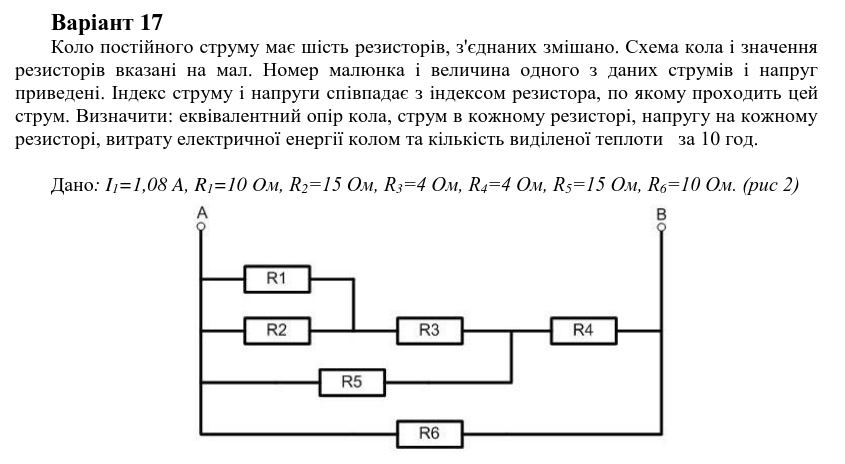
\includegraphics[scale=0.6]{v}
	\end{figure}
	
	\section*{Хід виконання}
	\begin{figure}[H]
		\centering
		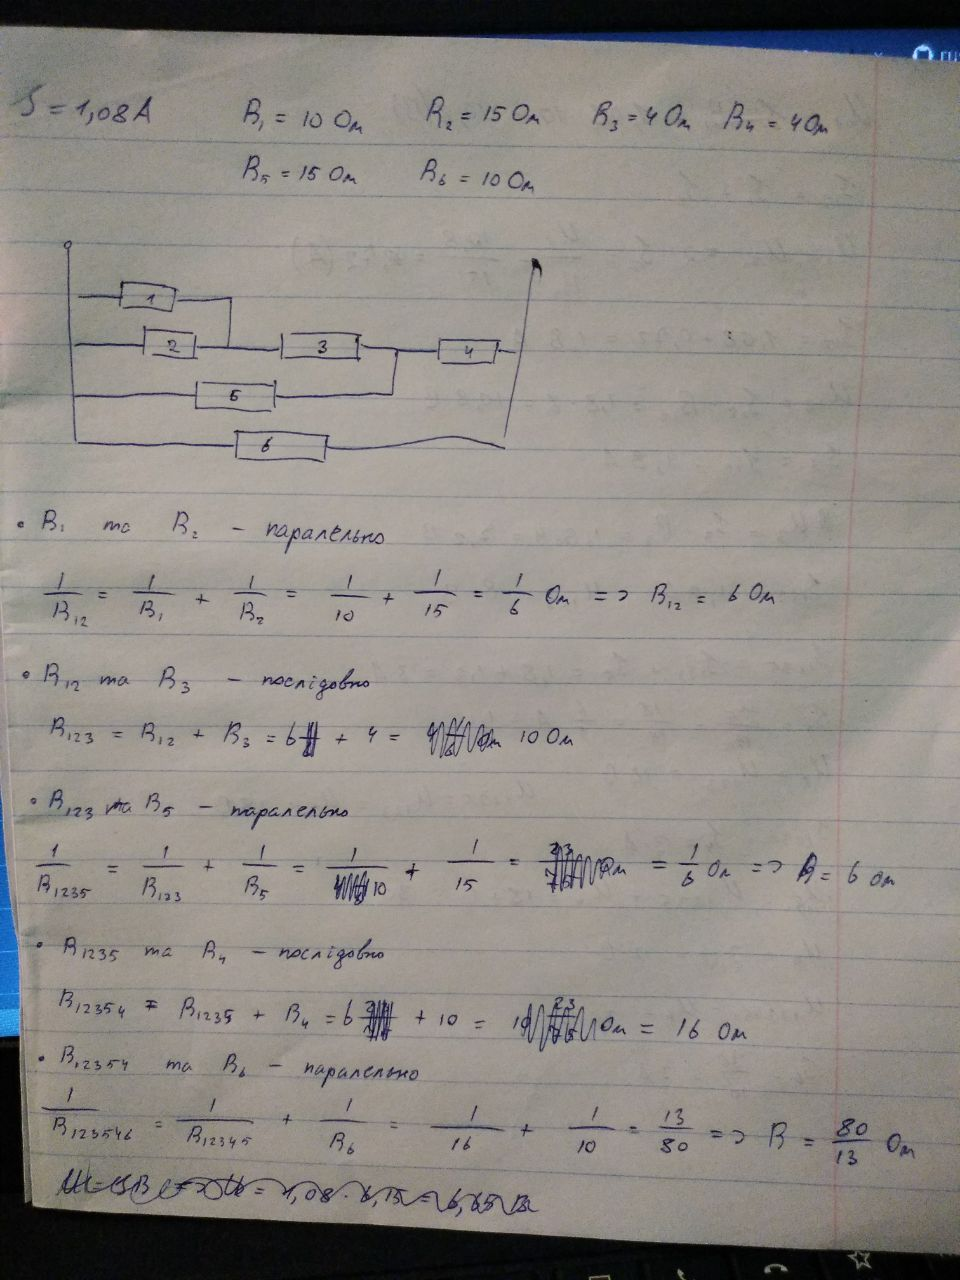
\includegraphics[scale=0.4]{11}
	\end{figure}
	
	\begin{figure}[H]
		\centering
		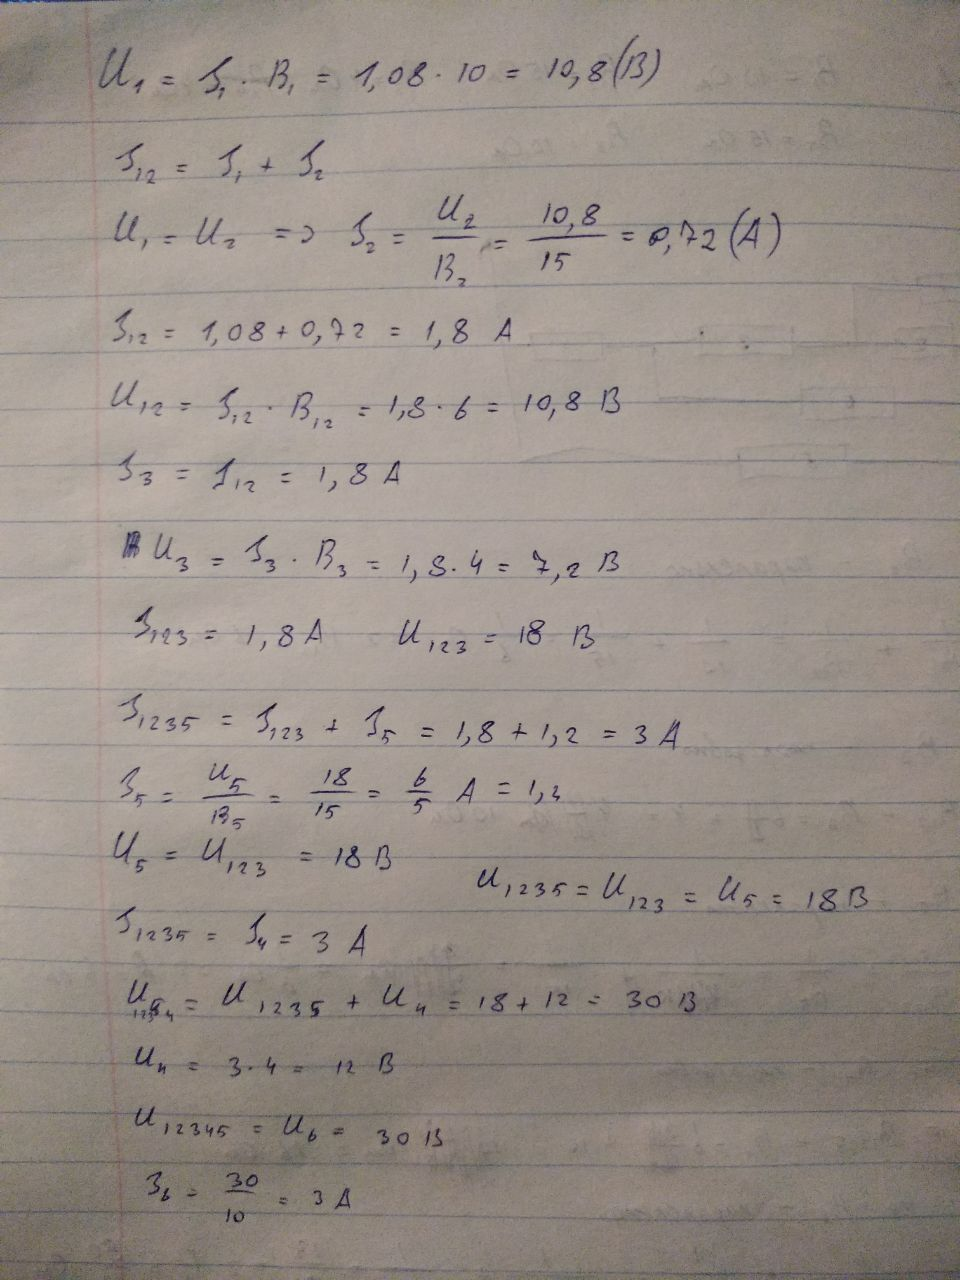
\includegraphics[scale=0.4]{22}
	\end{figure}
	
	Згідно отриманого завдання провів розрахунок кола постійного струму.
	\begin{Large}
		\begin{center}
			\begin{tabular}{ |c|c|c|c|c|c|c| } 
				\hline
				& $R_1$ & $R_2$ & $R_3$ & $R_4$ & $R_5$ & $R_6$ \\ 
				\hline
				I & 1.08 & 0.72 & 1.8 & 3 & 1.2 & 3 \\ 
				U & 10.8 & 10.8 & 7.2 & 12 & 18 & 30 \\ 
				R & 10 & 15 & 4 & 4 & 15 & 10 \\ 
				\hline
			\end{tabular}
		\end{center}
	\end{Large}
	Загальна напруга:
	\begin{equation}
		U = U_6 = \textup{30 В}\nonumber
	\end{equation}
	Загальний опір:
	\begin{gather}
		R_{12} = \frac{1}{\frac{1}{R_1} + \frac{1}{R_2}} = \textup{6 Ом}\notag\\
		R_{123} = R_{12} + R_3 = \textup{10 Ом}\notag\\
		R_{1235} = \frac{1}{\frac{1}{R_{123}} + \frac{1}{R_5}}\notag = \textup{6 Ом}\\
		R_{12345} = R_{1235} + R_4 = \textup{16 Ом}\notag\\
		R = \frac{1}{\frac{1}{R_{12345}} + \frac{1}{R_6}}= \frac{80}{13}=\textup{6.15 Ом}\notag
	\end{gather}
	Витрачена електрична енергія:
	\begin{gather}
		P=U\cdot I = 30\cdot6=\textup{180 Вт}\notag\\
		W=P\cdot t = 180\cdot 3600 = 648 \textup{ КВт}\cdot \textup{год}\notag
	\end{gather}
	Виділення теплоти за 10 год:
	\begin{gather}
		Q=I^2Rt=6^2\cdot6.15\cdot36000=\textup{7.9704 МДж}\notag
	\end{gather}

	\begin{figure}[H]
		\centering
		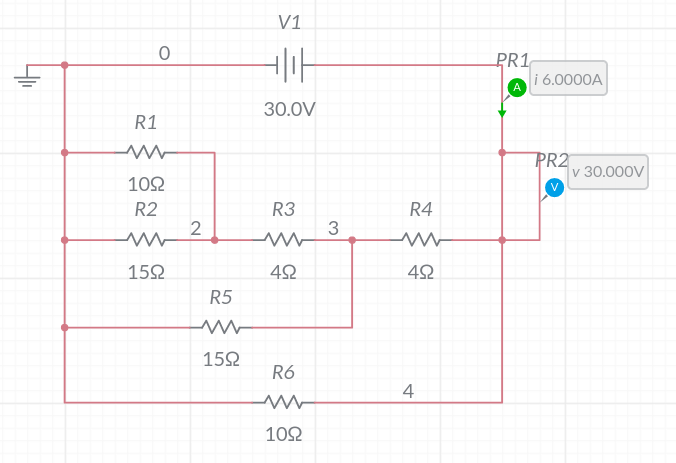
\includegraphics[scale=0.6]{1}
		\caption{Схема в середовищі Multisim Live}
	\end{figure}

	\section*{Висновки}
Під час виконання лабораторної роботи я ознайомився з програмним продуктом
	Multisim Live. Навчився складати кола постійного струму у програмі Multisim
	Live. Навчився обраховувати параметри кола постійного струму.
	    
\end{normalsize}
\end{document}
